\chapter{जीनोम की क्षति और कैंसर}\label{ch:g11:cancer}

सूक्ष्मदर्शी के नीचे स्वस्थ आँत की परत की कोई फाँक व्यवस्था की तस्वीर है:
सुथरी परतों में \omterm{def:g10:cells-common-unit:cell}{कोशिकाएँ}, हर एक में एक मामूली \omterm{def:g10:cells-common-unit:organelle}{केंद्रक}, परत के नीचे विभाजित
होती हुईं और ऊपर मरती हुईं, क़दम से क़दम मिलाकर। उसी फाँक में कुछ ही
मिलीमीटर दूर \omterm{def:g10:cells-common-unit:cell}{कोशिकाओं} का एक टुकड़ा क़तार तोड़ चुका है: भीड़ भरा, बेढंगा,
विशाल गहरे \omterm{def:g10:cells-common-unit:organelle}{केंद्रकों} वाला, कहीं भी विभाजित होता और नीचे के ऊतक में घुसता
हुआ। उस टुकड़े की हर \omterm{def:g10:cells-common-unit:cell}{कोशिका} उसी एक \omterm{def:g10:cells-common-unit:cell}{कोशिका} से उतरी है जिसने कुछ साल पहले
कोई ऐसा \omterm{def:g11:mutations:mutation}{उत्परिवर्तन} पाया जो उसे तब विभाजित होने देता था जब उसे नहीं होना
चाहिए था --- और फिर, सालों में, कुछ और भी। यह अध्याय इस बारे में है कि
\omterm{def:g11:cell-cycle-mitosis:cycle}{कोशिका चक्र} के नियंत्रण चूकते कैसे हैं, उन्हें नुक़सान क्या पहुँचाता है,
और पहले तथा बाद में क्या किया जा सकता है।

\section{तब विभाजित होना जब नहीं होना चाहिए}

\begin{definition}[कैंसर]\label{def:g11:cancer:cancer}
\emph{कैंसर}\index{कैंसर} \omterm{def:g10:cells-common-unit:cell}{कोशिकाओं} की वह आबादी है जो उन नियंत्रणों के बिना
विभाजित होती है जो सामान्य \omterm{def:g10:cells-common-unit:cell}{कोशिकाओं} का विभाजन सीमित रखते हैं, और जो
आसपास के ऊतकों में घुस जाती है। वह उसी एक \omterm{def:g10:cells-common-unit:cell}{कोशिका} से शुरू होता है जिसके
\omterm{def:g10:universal-dna:information}{DNA} में \omterm{def:g11:cell-cycle-mitosis:cycle}{कोशिका चक्र} को नियंत्रित करते \omterm{def:g10:universal-dna:gene}{जीनों} के \omterm{def:g11:mutations:mutation}{उत्परिवर्तन} जमा हो चुके
हों; और उस \omterm{def:g10:cells-common-unit:cell}{कोशिका} के वंशज \emph{अर्बुद}\index{अर्बुद} बना लेते हैं। जो
अर्बुद अपनी जगह सीमित रहे वह \emph{सौम्य} है; और जिसकी \omterm{def:g10:cells-common-unit:cell}{कोशिकाएँ} पड़ोसी
ऊतक में घुस जाएँ तथा रक्त या लसीका से चलकर कहीं और नए अर्बुद बसा दें
(\emph{विक्षेप}), वह \emph{दुर्दम} है।
\end{definition}

\begin{proposition}[कैंसर जीनोम का रोग है]\label{prop:g11:cancer:genome}
किसी \omterm{def:g11:cancer:cancer}{अर्बुद} की \omterm{def:g10:cells-common-unit:cell}{कोशिकाएँ} ऐसे \omterm{def:g11:mutations:mutation}{उत्परिवर्तन} ढोती हैं जो उसके मालिक की बाक़ी
\omterm{def:g10:cells-common-unit:cell}{कोशिकाओं} में नहीं हैं: यानी कायिक \omterm{def:g11:mutations:mutation}{उत्परिवर्तन}, जो किसी एक \omterm{def:g10:cells-common-unit:cell}{कोशिका} में उठे
और उसके वंशजों को विरासत में मिले। वह \omterm{def:g11:cancer:cancer}{अर्बुद} एक \emph{क्लोन} है, और वह
विकसित होता जाता है --- जो \omterm{def:g10:cells-common-unit:cell}{कोशिकाएँ} तेज़ विभाजित हों या बेहतर बचें वे
क़ब्ज़ा जमा लेती हैं, और बाद के \omterm{def:g11:mutations:mutation}{उत्परिवर्तन} घुसने तथा फैलने की क्षमता जोड़
देते हैं।
\end{proposition}
\begin{proof}[साक्ष्य]
\omterm{def:g11:cancer:cancer}{अर्बुद} \omterm{def:g10:cells-common-unit:cell}{कोशिकाओं} के \omterm{def:g10:universal-dna:information}{DNA} का अनुक्रमण उसी रोगी की सामान्य \omterm{def:g10:cells-common-unit:cell}{कोशिकाओं} के साथ रखकर
करने पर हज़ारों फ़र्क़ मिलते हैं, जो सब \omterm{def:g11:cancer:cancer}{अर्बुद} में हैं और कोई भी स्वस्थ ऊतक
में नहीं; और अर्बुद-दर-अर्बुद वही चंद \omterm{def:g10:universal-dna:gene}{जीन} उत्परिवर्तित मिलते हैं। किसी
स्त्री की हर \omterm{def:g11:cancer:cancer}{अर्बुद} \omterm{def:g10:cells-common-unit:cell}{कोशिका} उसके दोनों X \omterm{def:g10:universal-dna:information}{गुणसूत्रों} में से वही एक बंद किए
रहती है --- यानी अकेली एक \omterm{def:g10:cells-common-unit:cell}{कोशिका} से उतरने का निशान। और \omterm{def:g11:mutations:mutagen}{उत्परिवर्तजन}
\omterm{def:g11:cancer:carcinogen}{कैंसरजन} भी हैं: जो कारक \omterm{def:g11:mutations:mutation}{उत्परिवर्तन} की दर बढ़ाते हैं
(\cref{ch:g11:mutations}) वे दशकों की देरी के साथ \omterm{def:g11:cancer:cancer}{कैंसर} की दर भी बढ़ा देते
हैं।
\end{proof}

\begin{omfigure}
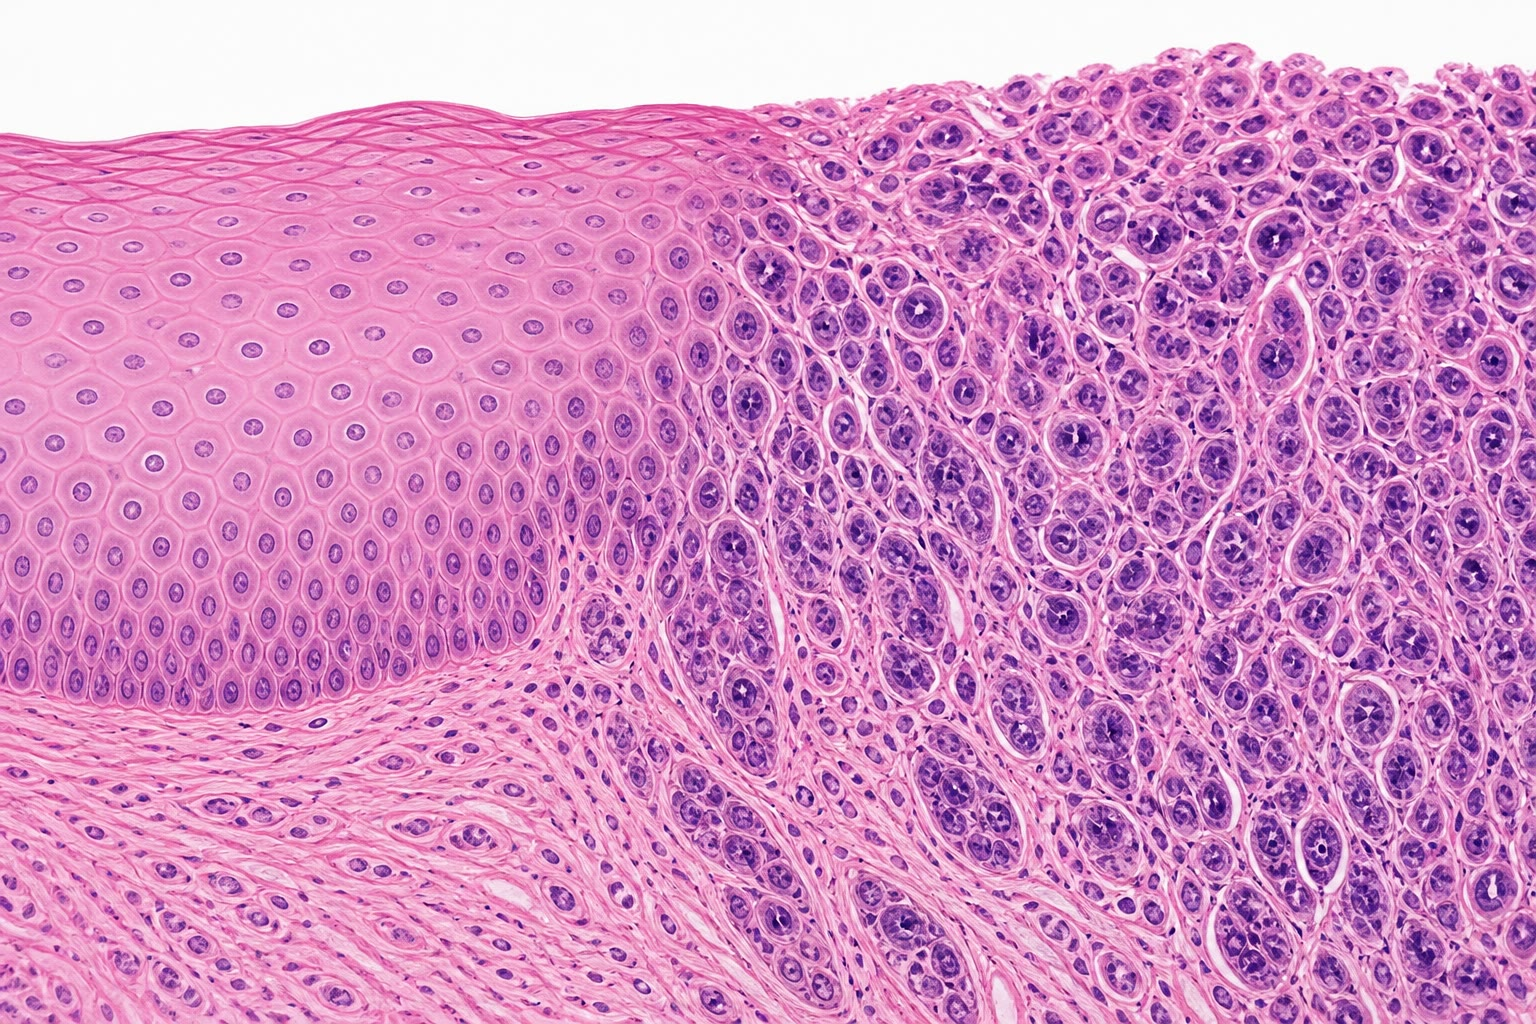
\includegraphics[width=0.62\linewidth]{images/book2/ai/g11-cancer-histology.jpg}

{\small रंगी हुई ऊतक की एक काट: बाईं ओर सुथरी परतों में व्यवस्थित
\omterm{def:g10:cells-common-unit:cell}{कोशिकाएँ}; और दाईं ओर बड़े, बेढंगे \omterm{def:g10:cells-common-unit:organelle}{केंद्रकों} वाली भीड़ भरी \omterm{def:g10:cells-common-unit:cell}{कोशिकाओं} का एक
अव्यवस्थित पिंड, जो ऊतक में घुसता जा रहा है। इन दोनों के बीच की सरहद ही
\omterm{def:g11:cancer:cancer}{अर्बुद} की सरहद है।}
\end{omfigure}

\section{गति और ब्रेक}

\begin{proposition}[दो तरह के जीन चक्र को नियंत्रित करते हैं]\label{prop:g11:cancer:genes}
किसी \omterm{def:g10:cells-common-unit:cell}{कोशिका} के विभाजित होने का फ़ैसला ऐसे \omterm{def:g11:gene-expression:protein}{प्रोटीन} करते हैं जो किसी गाड़ी के
गति-यंत्र और ब्रेक जैसा काम करते हैं।
\begin{itemize}
  \item \emph{प्रोटो-ऑन्कोजीन}\index{प्रोटो-ऑन्कोजीन} ऐसे प्रोटीनों के
        कूट हैं जो वृद्धि का कोई संकेत आते ही \omterm{def:g10:cells-common-unit:cell}{कोशिका} को चक्र में धकेल देते
        हैं --- यानी वृद्धि-संकेतों के ग्राही, और वे कड़ियाँ जो उस संकेत
        को \omterm{def:g10:cells-common-unit:organelle}{केंद्रक} तक ढोती हैं। जो \omterm{def:g11:mutations:mutation}{उत्परिवर्तन} ऐसे \omterm{def:g11:gene-expression:protein}{प्रोटीन} को हमेशा के लिए
        सक्रिय छोड़ दे वह उस \omterm{def:g10:universal-dna:gene}{जीन} को \emph{ऑन्कोजीन} बना देता है: यानी
        गति-यंत्र दबा हुआ जाम। इसके लिए एक ही उत्परिवर्ती \omterm{def:g10:universal-dna:gene}{युग्मविकल्पी} काफ़ी है।
  \item \emph{अर्बुद-दमनकारी जीन}\index{अर्बुद-दमनकारी जीन} ऐसे प्रोटीनों
        के कूट हैं जो \omterm{def:g10:universal-dna:information}{DNA} क्षतिग्रस्त होने पर चक्र रोक देते हैं ---
        S से पहले और \omterm{def:g11:cell-cycle-mitosis:cycle}{समसूत्री विभाजन} से पहले के जाँच-बिंदुओं पर --- और जो
        मरम्मत शुरू कराते हैं, या यदि क्षति मरम्मत से परे हो तो \omterm{def:g10:cells-common-unit:cell}{कोशिका} का
        आत्म-विनाश। जो \omterm{def:g11:mutations:mutation}{उत्परिवर्तन} ऐसे \omterm{def:g11:gene-expression:protein}{प्रोटीन} को निष्क्रिय कर दे वह एक
        ब्रेक हटा देता है; और चूँकि \omterm{def:g10:cells-common-unit:cell}{कोशिका} के पास दो \omterm{def:g10:universal-dna:gene}{युग्मविकल्पी} हैं, इसलिए
        दोनों खोने पड़ते हैं।
\end{itemize}
सबसे जाना-पहचाना दमनकारी, यानी \omterm{def:g11:gene-expression:protein}{प्रोटीन} p53, सारे मानव \omterm{def:g11:cancer:cancer}{कैंसरों} के आधे में
निष्क्रिय पाया जाता है।
\end{proposition}
\admitted

\begin{omfigure}
\begin{tikzpicture}[font=\small, >=Stealth,
  b/.style={draw, rounded corners, align=center, text width=2.8cm, minimum height=1.0cm}]
  \node[b, fill=omMeth!15] (sig) at (0,1.2) {दूसरी कोशिकाओं से\\ वृद्धि का संकेत};
  \node[b, fill=omMeth!15] (onc) at (3.8,1.2) {प्रोटो-ऑन्कोजीन के\\ प्रोटीन उसे आगे ढोते हैं};
  \node[b, fill=omDef!15] (cyc) at (7.6,1.2) {कोशिका चक्र में\\ घुसती है};
  \node[b, fill=omDef!15] (div) at (11.4,1.2) {विभाजन};
  \draw[->, thick] (sig) -- (onc); \draw[->, thick] (onc) -- (cyc); \draw[->, thick] (cyc) -- (div);
  \node[b, fill=omThm!12] (dam) at (3.8,-1.4) {DNA की क्षति\\ पकड़ी गई};
  \node[b, fill=omThm!12, text width=3.1cm] (p53) at (7.6,-1.4) {अर्बुद-दमनकारी\\ प्रोटीन (p53\dots)};
  \node[b, fill=omThm!12, text width=3.4cm] (halt) at (11.4,-1.4) {चक्र रोकते हैं;\\ मरम्मत, या आत्म-विनाश};
  \draw[->, thick] (dam) -- (p53); \draw[->, thick] (p53) -- (halt);
  \draw[thick, omThm] (11.4,-0.85) -- (11.4,0.5);
  \draw[thick, omThm] (11.1,0.5) -- (11.7,0.5);
  \node[anchor=east, font=\scriptsize, omThm, align=right] at (11.0,-0.2) {ब्रेक};
  \node[anchor=west, font=\scriptsize, omMeth!60!black] at (0.2,2.05) {गति-यंत्र};
\end{tikzpicture}

{\small विभाजन के नियंत्रण। \omterm{prop:g11:cancer:genes}{प्रोटो-ऑन्कोजीन} के \omterm{def:g11:gene-expression:protein}{प्रोटीन} वृद्धि के संकेत आगे
ढोते हैं और \omterm{def:g10:cells-common-unit:cell}{कोशिका} को चक्र में धकेलते हैं (गति-यंत्र); और
अर्बुद-दमनकारी \omterm{def:g11:gene-expression:protein}{प्रोटीन} \omterm{def:g10:universal-dna:information}{DNA} क्षतिग्रस्त होने पर उसे रोक देते हैं (ब्रेक)।
ऑन्कोजीन चालू जाम हुआ गति-यंत्र है; और खोया हुआ दमनकारी हटा दिया गया
ब्रेक।}
\end{omfigure}

\begin{example}[दो जाने-पहचाने जीन]\label{ex:g11:cancer:genes}
वृद्धि के किसी संकेत का ग्राही बहुत-सी \omterm{def:g10:cells-common-unit:cell}{कोशिकाओं} की झिल्ली में बैठा होता है;
और उसके \omterm{def:g10:universal-dna:gene}{जीन} में एक ही प्रतिस्थापन उसे बाहर बिना किसी संकेत के भी लगातार
संकेत देता रहने वाला बना देता है --- यानी वह ऑन्कोजीन, जो बृहदांत्र और
फेफड़े के एक-तिहाई \omterm{def:g11:cancer:cancer}{कैंसरों} में मिलता है। दूसरी ओर p53 का \omterm{def:g10:universal-dna:gene}{जीन} हर संभव तरीक़े
से निष्क्रिय किया जाता है: उसका आकार बदलने वाले प्रतिस्थापनों से, विलोपनों
से, समय से पहले किसी विराम से। जिस \omterm{def:g10:cells-common-unit:cell}{कोशिका} ने p53 खो दिया वह अपना \omterm{def:g10:universal-dna:information}{DNA} नक़ल
करने से पहले उसकी मरम्मत के लिए रुकती नहीं, इसलिए वह और \omterm{def:g11:mutations:mutation}{उत्परिवर्तन} तेज़ी
से जमा करती है: यानी वह ब्रेक खोना पूरी प्रक्रिया को तेज़ कर देता है।
\end{example}

\section{कई क़दम, कई साल}

\begin{proposition}[कैंसर कई क़दमों की प्रक्रिया है]\label{prop:g11:cancer:multistep}
अकेला एक \omterm{def:g11:mutations:mutation}{उत्परिवर्तन} \omterm{def:g11:cancer:cancer}{कैंसर} नहीं बनाता। किसी \omterm{def:g10:cells-common-unit:cell}{कोशिका} को कई जमा करने पड़ते
हैं --- आमतौर पर एक ऑन्कोजीन सक्रिय और दो या अधिक दमनकारी खोए हुए --- और
हर अगला \omterm{def:g11:mutations:mutation}{उत्परिवर्तन}, उस क्लोन का बढ़ना तेज़ करके, उन \omterm{def:g10:cells-common-unit:cell}{कोशिकाओं} की संख्या
बढ़ा देता है जिनमें अगला हो सकता है। इस क्रम में साल से लेकर दशकों तक लगते
हैं, और इसीलिए अधिकांश \omterm{def:g11:cancer:cancer}{कैंसरों} की घटना-दर उम्र के साथ तीखेपन से चढ़ती है,
तथा इसीलिए किसी \omterm{def:g11:cancer:carcinogen}{कैंसरजन} का असर संपर्क के बीस या तीस साल बाद उभरता है।
\end{proposition}
\begin{proof}[साक्ष्य]
बृहदांत्र में ये चरण देखे जा सकते हैं: एक दमनकारी \omterm{def:g11:mutations:mutation}{उत्परिवर्तन} ढोता छोटा
सौम्य पॉलिप; उसके ऊपर एक ऑन्कोजीन जुड़ा बड़ा पॉलिप; और उसके ऊपर p53 भी खोया
हुआ, यानी घुसपैठ करता \omterm{def:g11:cancer:cancer}{अर्बुद} --- यानी दस से बीस साल में क़रीब चार से छह
\omterm{def:g11:mutations:mutation}{उत्परिवर्तनों} का एक क्रम, जिसका हर चरण अगले की \omterm{def:g10:cells-common-unit:cell}{कोशिकाओं} में मिलता है।
\omterm{def:g11:cancer:cancer}{कैंसर} की घटना-दर मोटे तौर पर उम्र की पाँचवीं घात के हिसाब से चढ़ती है,
यानी वही वक्र जिसकी उम्मीद तब होती है जब किसी एक \omterm{def:g10:cells-common-unit:cell}{कोशिका} में लगभग पाँच या
छह स्वतंत्र विरली घटनाएँ घटनी हों। और जिन लोगों को किसी दमनकारी \omterm{def:g10:universal-dna:gene}{जीन} का एक
उत्परिवर्ती \omterm{def:g10:universal-dna:gene}{युग्मविकल्पी} विरासत में मिलता है उनमें उससे मेल खाता \omterm{def:g11:cancer:cancer}{कैंसर} जल्दी और
अधिक बार होता है, क्योंकि उनकी हर \omterm{def:g10:cells-common-unit:cell}{कोशिका} में एक क़दम पहले ही उठ चुका है।
\end{proof}

\begin{omfigure}
\begin{tikzpicture}[font=\small, >=Stealth]
  \tikzset{c/.style={circle, draw, inner sep=0, minimum size=0.28cm}}
  % stage 1: one normal cell mutates
  \foreach \x in {0,0.35,...,1.05} \foreach \y in {0,0.35,0.7} \node[c, fill=omDef!15] at (\x,\y) {};
  \node[c, fill=omProp!60] at (0.7,0.35) {};
  \node[anchor=north, align=center, text width=2.4cm] at (0.5,-0.4) {एक कोशिका को\\ उत्परिवर्तन 1 मिलता है};
  \draw[->, thick] (1.5,0.35) -- (2.3,0.35) node[midway, above, font=\scriptsize] {साल};
  % stage 2: clone
  \begin{scope}[xshift=2.7cm]
    \foreach \x in {0,0.35,...,1.4} \foreach \y in {0,0.35,0.7} \node[c, fill=omDef!15] at (\x,\y) {};
    \foreach \x in {0.35,0.7,1.05} \foreach \y in {0.35,0.7} \node[c, fill=omProp!60] at (\x,\y) {};
    \node[c, fill=omThm!70] at (0.7,0.35) {};
    \node[anchor=north, align=center, text width=2.6cm] at (0.7,-0.4) {उसका क्लोन बढ़ता है;\\ एक कोशिका को\\ उत्परिवर्तन 2 मिलता है};
  \end{scope}
  \draw[->, thick] (4.6,0.35) -- (5.4,0.35) node[midway, above, font=\scriptsize] {साल};
  % stage 3: larger clone
  \begin{scope}[xshift=5.8cm]
    \foreach \x in {0,0.35,...,1.75} \foreach \y in {0,0.35,0.7,1.05} \node[c, fill=omProp!60] at (\x,\y) {};
    \foreach \x in {0.35,0.7,1.05,1.4} \foreach \y in {0.35,0.7} \node[c, fill=omThm!70] at (\x,\y) {};
    \node[c, fill=black!70] at (0.7,0.35) {};
    \node[anchor=north, align=center, text width=2.8cm] at (0.9,-0.4) {सबसे तेज़ क्लोन में\\ उत्परिवर्तन 3:\\ घुसपैठी कैंसर};
  \end{scope}
  \draw[->, thick] (8.0,0.35) -- (8.8,0.35) node[midway, above, font=\scriptsize] {साल};
  \begin{scope}[xshift=9.2cm]
    \foreach \x in {0,0.35,...,2.1} \foreach \y in {0,0.35,0.7,1.05} \node[c, fill=omThm!70] at (\x,\y) {};
    \foreach \x in {0.35,0.7,...,1.75} \foreach \y in {0.35,0.7} \node[c, fill=black!70] at (\x,\y) {};
    \node[anchor=north, align=center, text width=2.6cm] at (1.05,-0.4) {अर्बुद: क्लोनों\\ का एक क्लोन};
  \end{scope}
\end{tikzpicture}

{\small क्लोनी विकास। विभाजन तेज़ करता हर \omterm{def:g11:mutations:mutation}{उत्परिवर्तन} उस क्लोन को बड़ा कर
देता है जिसमें अगला \omterm{def:g11:mutations:mutation}{उत्परिवर्तन} हो सकता है; और ऐसे कई क़दमों के बाद, सालों
में, एक वंशक्रम हर नियंत्रण खो चुका होता है। \omterm{def:g11:cancer:cancer}{अर्बुद} क्लोनों का एक घोंसला
है, जिसमें सबसे नया सबसे पुराने के भीतर बैठा है।}
\end{omfigure}

\begin{omfigure}
\begin{tikzpicture}
\begin{axis}[
  width=0.86\linewidth, height=5.6cm,
  axis x line=bottom, axis y line=left,
  xmin=0, xmax=90, ymin=0, ymax=3200,
  xlabel={उम्र (साल)}, ylabel={प्रति 100\,000 प्रति वर्ष नए कैंसर},
  xlabel style={font=\small, at={(axis description cs:0.5,-0.12)}, anchor=north},
  ylabel style={font=\small},
  tick label style={font=\small}, xtick={0,20,40,60,80}, ytick={0,1000,2000,3000},
]
\addplot[thick, omThm, mark=*, mark size=1.4pt] coordinates
  {(5,20) (15,25) (25,45) (35,110) (45,300) (55,700) (65,1500) (75,2400) (85,3000)};
\end{axis}
\end{tikzpicture}

{\small उम्र के सापेक्ष सारे \omterm{def:g11:cancer:cancer}{कैंसरों} की सालाना घटना-दर (राष्ट्रीय पंजियों
से गोल की हुई)। यह चढ़ाई समानुपाती से कहीं तीखी है: 35 से 70 तक उम्र दोगुनी
होती है और घटना-दर बीस गुना चढ़ जाती है --- यानी उन कई विरली घटनाओं का
निशान जिन्हें एक ही \omterm{def:g10:cells-common-unit:cell}{कोशिका} में घटना है।}
\end{omfigure}

\section{जीनोम को नुक़सान क्या पहुँचाता है}

\begin{definition}[कैंसरजन]\label{def:g11:cancer:carcinogen}
\emph{कैंसरजन}\index{कैंसरजन} वह कारक है जो \omterm{def:g11:cancer:cancer}{कैंसर} का जोखिम बढ़ा देता है।
अधिकांश \omterm{def:g11:mutations:mutagen}{उत्परिवर्तजन} हैं: धूप की पराबैंगनी (त्वचा के \omterm{def:g11:cancer:cancer}{कैंसर}), तंबाकू के
धुएँ का तारकोल (फेफड़ा, मुँह, मूत्राशय), आयनकारी विकिरण, एस्बेस्टस के
रेशे, शराब, कुछ फफूँदें। कुछ और तरह से काम करते हैं: कुछ विषाणु ऐसे \omterm{def:g10:universal-dna:gene}{जीन}
ढोते हैं जो \omterm{def:g10:cells-common-unit:cell}{कोशिका} के ब्रेक जाम कर देते हैं --- मानव पैपिलोमा विषाणु
गर्भाशय ग्रीवा के लगभग सारे \omterm{def:g11:cancer:cancer}{कैंसर} करते हैं, और यकृतशोथ के विषाणु यकृत के
बहुत-से \omterm{def:g11:cancer:cancer}{कैंसर} --- और लगातार बना शोथ या ऐसे हॉर्मोन जो किसी ऊतक को विभाजित
होते रखें, उन विभाजनों की संख्या बढ़ा देते हैं जिनमें \omterm{def:g11:mutations:mutation}{उत्परिवर्तन} हो सकते
हैं।
\end{definition}

\begin{omfigure}
\begin{tikzpicture}
\begin{axis}[
  width=0.86\linewidth, height=5.4cm,
  axis x line=bottom, axis y line=left,
  xmin=0, xmax=45, ymin=0, ymax=30,
  xlabel={प्रति दिन सिगरेट}, ylabel={फेफड़े के कैंसर का सापेक्ष जोखिम},
  xlabel style={font=\small, at={(axis description cs:0.5,-0.12)}, anchor=north},
  ylabel style={font=\small},
  tick label style={font=\small}, xtick={0,10,20,30,40}, ytick={0,5,10,15,20,25,30},
]
\addplot[thick, omThm, mark=*, mark size=1.5pt] coordinates
  {(0,1) (5,6) (10,10) (15,14) (20,17) (25,20) (30,22) (40,25)};
\end{axis}
\end{tikzpicture}

{\small दशकों तक प्रति दिन पी गई सिगरेटों की संख्या के सापेक्ष, किसी
धूम्रपान न करने वाले के मुक़ाबले फेफड़े के \omterm{def:g11:cancer:cancer}{कैंसर} का जोखिम (लंबी अवधि के
अध्ययनों से गोल किया हुआ)। जोखिम ख़ुराक के साथ चढ़ता है, ठीक जैसा फेफड़ों
तक पहुँचाए गए किसी \omterm{def:g11:mutations:mutagen}{उत्परिवर्तजन} से अपेक्षित है।}
\end{omfigure}

\begin{example}[तंबाकू]\label{ex:g11:cancer:tobacco}
धुआँ क़रीब सत्तर \omterm{def:g11:cancer:carcinogen}{कैंसरजन} ढोता है; और बेंज़ोपाइरीन, \omterm{def:g10:cells-common-unit:cell}{कोशिकाओं} के अपने ही
एंजाइमों से सक्रिय होकर, ग्वानीनों से चिपक जाता है और उन्हीं स्थानों पर
प्रतिस्थापन कर देता है। किसी धूम्रपान करने वाले के फेफड़े के \omterm{def:g11:cancer:cancer}{अर्बुद} का p53
\omterm{def:g10:universal-dna:gene}{जीन} आमतौर पर ठीक वैसा ही प्रतिस्थापन ढोता है, उन चंद स्थानों में से किसी एक
पर जहाँ बेंज़ोपाइरीन सबसे आसानी से बँधता है --- यानी वह \omterm{def:g11:mutations:mutagen}{उत्परिवर्तजन}
अनुक्रम में अपना निशान छोड़ जाता है। सिगरेटों से पहले फेफड़े का \omterm{def:g11:cancer:cancer}{कैंसर} एक
विरली चीज़ थी; धूम्रपान दस में नौ मामले करता है, और छोड़ देने से जोखिम दस
साल में आधा हो जाता है, क्योंकि शुरुआती क़दम ढोती \omterm{def:g10:cells-common-unit:cell}{कोशिकाएँ} धीरे-धीरे बदल दी
जाती हैं।
\end{example}

\begin{proposition}[विरासत में मिली प्रवृत्ति]\label{prop:g11:cancer:inherited}
\omterm{def:g11:cancer:cancer}{कैंसर} ख़ुद विरासत में नहीं मिलता --- वह कायिक \omterm{def:g11:mutations:mutation}{उत्परिवर्तनों} का रोग है ---
पर किसी दमनकारी \omterm{def:g10:universal-dna:gene}{जीन} का उत्परिवर्ती \omterm{def:g10:universal-dna:gene}{युग्मविकल्पी} मिल सकता है। जिस व्यक्ति को ऐसे
\omterm{def:g10:universal-dna:gene}{जीन} का एक बेकार \omterm{def:g10:universal-dna:gene}{युग्मविकल्पी} विरासत में मिला हो, उसके शरीर की हर \omterm{def:g10:cells-common-unit:cell}{कोशिका} में एक
क़दम उठ चुका है; और किसी भी \omterm{def:g10:cells-common-unit:cell}{कोशिका} में दूसरे \omterm{def:g10:universal-dna:gene}{युग्मविकल्पी} का अकेला एक कायिक
\omterm{def:g11:mutations:mutation}{उत्परिवर्तन} वह हानि पूरी कर देता है, जबकि बाक़ी लोगों में दो चाहिए। इसका
नतीजा है उन \omterm{def:g11:cancer:cancer}{कैंसरों} का ऊँचा जोखिम, और जीवन में जल्दी: स्तन \omterm{def:g11:cancer:cancer}{कैंसर} के किसी
एक ख़ास \omterm{def:g10:universal-dna:gene}{जीन} का उत्परिवर्ती \omterm{def:g10:universal-dna:gene}{युग्मविकल्पी} ढोती स्त्रियों में से क़रीब 70\% को वह
रोग होता है, जबकि आम तौर पर 12\% को।
\end{proposition}
\admitted

\section{रोकथाम, पहचान, इलाज}

\begin{method}[जोखिम घटाना]\label{met:g11:cancer:prevention}
चूँकि \omterm{def:g11:cancer:cancer}{कैंसरों} के पीछे के अधिकांश \omterm{def:g11:mutations:mutation}{उत्परिवर्तन} पहचाने जा सकने वाले संपर्कों
से आते हैं, और चूँकि यह प्रक्रिया सालों लेती है, इसलिए \omterm{def:g11:cancer:cancer}{कैंसर} बड़े हिस्से
में रोका और पकड़ा जा सकता है।
\begin{enumerate}
  \item \emph{\omterm{def:g11:mutations:mutagen}{उत्परिवर्तजनों} से बचिए}: कोई तंबाकू नहीं (\omterm{def:g11:cancer:cancer}{कैंसर} से होने
        वाली एक-तिहाई मौतें), शराब कम, धूप से बचाव, कोई ग़ैर-ज़रूरी
        विकिरण नहीं।
  \item \omterm{def:g11:cancer:cancer}{कैंसर} करने वाले विषाणुओं के ख़िलाफ़ \emph{टीका लगवाइए}: संपर्क से
        पहले दिया गया पैपिलोमा विषाणु का टीका गर्भाशय ग्रीवा के लगभग सारे
        \omterm{def:g11:cancer:cancer}{कैंसर} रोक देता है।
  \item \emph{छानबीन कीजिए}: \omterm{def:g11:cancer:cancer}{अर्बुद} को पॉलिप वाली अवस्था में ही पकड़िए ---
        ग्रीवा की लेप जाँच, बृहदांत्रदर्शन, स्तन-चित्रण --- जब उसे हटाना
        सरल और पूरा इलाज दोनों हो।
  \item \emph{परिवार को जानिए}: विरासत में मिली कोई प्रवृत्ति जल्दी और
        क़रीबी निगरानी माँगती है।
\end{enumerate}
\end{method}

\begin{example}[इलाज और उनके निशाने]\label{ex:g11:cancer:treatments}
शल्यक्रिया उस \omterm{def:g11:cancer:cancer}{अर्बुद} को हटा देती है जो फैला न हो। विकिरण चिकित्सा पुंज में
आती \omterm{def:g10:cells-common-unit:cell}{कोशिकाओं} का \omterm{def:g10:universal-dna:information}{DNA} मरम्मत से परे तोड़ देती है और ख़ासकर विभाजित होती
\omterm{def:g10:cells-common-unit:cell}{कोशिकाएँ} मार देती है। रसायन चिकित्सा ऐसी दवाएँ इस्तेमाल करती है जो
प्रतिकृतिकरण या तर्कु रोक देती हैं (\cref{ch:g11:cell-cycle-mitosis}):
लगातार विभाजित होती \omterm{def:g11:cancer:cancer}{अर्बुद} \omterm{def:g10:cells-common-unit:cell}{कोशिकाएँ} सामान्य \omterm{def:g10:cells-common-unit:cell}{कोशिकाओं} से तेज़ी से मरती हैं
--- पर तेज़ी से विभाजित होते सामान्य ऊतक भी (अस्थि मज्जा, आँत की परत,
बालों की जड़ें) झेलते हैं, और दुष्प्रभाव वहीं से आते हैं। और नए इलाज किसी
\omterm{def:g11:cancer:cancer}{अर्बुद} के उस ख़ास उत्परिवर्ती \omterm{def:g11:gene-expression:protein}{प्रोटीन} को निशाना बनाते हैं, या उस पर
प्रतिरक्षा तंत्र छोड़ देते हैं।
\end{example}

\begin{remark}[हम सब उसकी शुरुआत क्यों ढोते हैं]\label{rem:g11:cancer:everyone}
हर वयस्क \omterm{def:g11:cancer:cancer}{कैंसर} से जुड़े \omterm{def:g11:mutations:mutation}{उत्परिवर्तन} वाली \omterm{def:g10:cells-common-unit:cell}{कोशिकाओं} के क्लोन ढोता है ---
त्वचा में, आँत में, रक्त में --- जो कभी \omterm{def:g11:cancer:cancer}{कैंसर} बनते ही नहीं: बचे हुए ब्रेक
थामे रहते हैं, प्रतिरक्षा तंत्र सबसे बुरों को हटा देता है, और वह व्यक्ति
उससे पहले किसी और चीज़ से मर जाता है। \omterm{def:g11:cancer:cancer}{कैंसर} उस प्रक्रिया का कभी-कभार आने
वाला नतीजा है जो हर किसी में चलती है; और रोकथाम का लक्ष्य यह है कि किसी भी
एक \omterm{def:g10:cells-common-unit:cell}{कोशिका} में उठे क़दमों की संख्या ज़रूरी संख्या से नीचे बनी रहे।
\end{remark}

\section{अभ्यास}

\begin{exercise}[$\star$]\label{exo:g11:cancer:1}
\omterm{def:g11:cancer:cancer}{कैंसर}, \omterm{def:g11:cancer:cancer}{अर्बुद} और विक्षेप की परिभाषा दीजिए।
\end{exercise}

\begin{exercise}[$\star$]\label{exo:g11:cancer:2}
\omterm{prop:g11:cancer:genes}{प्रोटो-ऑन्कोजीन} क्या है, और उत्परिवर्तित होने पर वह क्या बन जाता है? एक ही
उत्परिवर्ती \omterm{def:g10:universal-dna:gene}{युग्मविकल्पी} क्यों काफ़ी है?
\end{exercise}

\begin{exercise}[$\star$]\label{exo:g11:cancer:3}
p53 जैसा कोई अर्बुद-दमनकारी \omterm{def:g11:gene-expression:protein}{प्रोटीन} क्या करता है? दोनों \omterm{def:g10:universal-dna:gene}{युग्मविकल्पी} क्यों खोने
पड़ते हैं?
\end{exercise}

\begin{exercise}[$\star$]\label{exo:g11:cancer:4}
चार \omterm{def:g11:cancer:carcinogen}{कैंसरजनों} के नाम लिखिए और उनमें से दो के लिए वह \omterm{def:g11:cancer:cancer}{कैंसर} भी जो वे करते हैं।
\end{exercise}

\begin{exercise}[$\star$]\label{exo:g11:cancer:5}
किसी \omterm{def:g11:cancer:cancer}{कैंसर} को क्लोन क्यों कहा जाता है?
\end{exercise}

\begin{exercise}[$\star\star$]\label{exo:g11:cancer:6}
उम्र वाले चित्र से 40 और 80 पर घटना-दर पढ़िए और गुणक निकालिए। उम्र के
गुणक 2 से तुलना कीजिए।
\end{exercise}

\begin{exercise}[$\star\star$]\label{exo:g11:cancer:7}
तंबाकू वाले चित्र से प्रति दिन 10 और 20 सिगरेट पर सापेक्ष जोखिम बताइए।
यदि किसी धूम्रपान न करने वाले का जीवन भर का जोखिम 1\% हो, तो प्रति दिन 20
पीने वाले का कितना है?
\end{exercise}

\begin{exercise}[$\star\star$]\label{exo:g11:cancer:8}
समझाइए कि जिस \omterm{def:g10:cells-common-unit:cell}{कोशिका} ने p53 खो दिया है वह किसी सामान्य \omterm{def:g10:cells-common-unit:cell}{कोशिका} से तेज़ी से
और \omterm{def:g11:mutations:mutation}{उत्परिवर्तन} क्यों जमा करती है।
\end{exercise}

\begin{exercise}[$\star\star$]\label{exo:g11:cancer:9}
किसी स्त्री को स्तन \omterm{def:g11:cancer:cancer}{कैंसर} के किसी दमनकारी \omterm{def:g10:universal-dna:gene}{जीन} का एक उत्परिवर्ती \omterm{def:g10:universal-dna:gene}{युग्मविकल्पी}
विरासत में मिलता है। ``क़दमों'' की भाषा में समझाइए कि उसका जोखिम ऊँचा और
उसके \omterm{def:g11:cancer:cancer}{कैंसर} जल्दी क्यों हैं; और उसकी बहनों के लिए वही होने की संभावना दो
में एक क्यों है।
\end{exercise}

\begin{exercise}[$\star\star$]\label{exo:g11:cancer:10}
रसायन चिकित्सा की दवाएँ बाल झड़ना, मितली और श्वेत रक्त \omterm{def:g10:cells-common-unit:cell}{कोशिकाओं} में गिरावट
क्यों करती हैं?
\end{exercise}

\begin{exercise}[$\star\star$]\label{exo:g11:cancer:11}
40 पर धूम्रपान छोड़ देने वाले को 60 पर, जारी रखने वाले के मुक़ाबले,
फेफड़े के \omterm{def:g11:cancer:cancer}{कैंसर} का आधा जोखिम रहता है। कई क़दमों वाले मॉडल से समझाइए कि
जोखिम गिरता तो है पर धूम्रपान न करने वाले जितना क्यों नहीं हो जाता।
\end{exercise}

\begin{exercise}[$\star\star\star$]\label{exo:g11:cancer:12}
मान लीजिए किसी \omterm{def:g11:cancer:cancer}{कैंसर} को 3 ख़ास \omterm{def:g11:mutations:mutation}{उत्परिवर्तन} चाहिए, और हर एक की प्रायिकता
प्रति \omterm{def:g10:cells-common-unit:cell}{कोशिका} विभाजन $10^{-7}$ है। किसी ऊतक की मूल \omterm{def:g10:cells-common-unit:cell}{कोशिकाएँ} जीवन भर में
$10^{12}$ बार विभाजित होती हैं। आँकिए कि पहला \omterm{def:g11:mutations:mutation}{उत्परिवर्तन} पाने वाली
\omterm{def:g10:cells-common-unit:cell}{कोशिकाओं} की अपेक्षित संख्या कितनी है; और क्लोन के फैलाव की मदद से समझाइए
कि तीनों के लिए सीधा गुणनफल $10^{-21}$ कहीं बहुत कम क्यों है।
\end{exercise}

\begin{exercise}[$\star\star\star$]\label{exo:g11:cancer:13}
कोई पैपिलोमा विषाणु ऐसा \omterm{def:g10:universal-dna:gene}{जीन} ढोता है जिसका \omterm{def:g11:gene-expression:protein}{प्रोटीन} p53 से बँधकर उसे
निष्क्रिय कर देता है। समझाइए कि वह विषाणु किसी मानव \omterm{def:g10:universal-dna:gene}{जीन} को उत्परिवर्तित
किए बिना \omterm{def:g11:cancer:cancer}{कैंसर} कैसे करता है, टीका उसे कैसे रोकता है, और संपर्क से पहले
टीका लगाना क्यों मायने रखता है।
\end{exercise}

\begin{exercise}[$\star\star\star$]\label{exo:g11:cancer:14}
50 की उम्र से हर दस साल पर बृहदांत्रदर्शन से बृहदांत्र के \omterm{def:g11:cancer:cancer}{कैंसर} की छानबीन
मिले हुए पॉलिप हटा देती है। कई क़दमों वाले मॉडल की मदद से समझाइए कि यह केवल
पकड़ने के बजाय \omterm{def:g11:cancer:cancer}{कैंसर} रोक क्यों देती है, और दस साल का अंतराल ठीक-ठाक क्यों
है।
\end{exercise}

\begin{exercise}[$\star\star\star$]\label{exo:g11:cancer:15}
``\omterm{def:g11:cancer:cancer}{कैंसर} बुढ़ापे का रोग है, इसलिए कुछ किया ही नहीं जा सकता।'' उम्र वाले
वक्र, \omterm{def:g11:cancer:carcinogen}{कैंसरजनों} की देरी, ज्ञात संपर्कों से जुड़े \omterm{def:g11:cancer:cancer}{कैंसरों} के अंश, और छानबीन
की मदद से एक अनुच्छेद में चर्चा कीजिए।
\end{exercise}

\section{समस्या: जीन में छूटा निशान}

\begin{problem}[{सप्ताहांत समस्या --- फेफड़े के किसी अर्बुद का अनुक्रमण:
उत्परिवर्तन गिने गए, धूम्रपान करने वाले का निशान पढ़ा गया, साल जोड़े गए, और
वह जोखिम जो एक सिगरेट ढोती है}]
\label{pb:g11:cancer:1}
35 साल तक रोज़ 20 सिगरेट पीने वाले एक ही रोगी के फेफड़े के \omterm{def:g11:cancer:cancer}{अर्बुद} और स्वस्थ
ऊतक, दोनों का अनुक्रमण होता है। वह \omterm{def:g11:cancer:cancer}{अर्बुद} $\num{5000}$ ऐसे कायिक
प्रतिस्थापन ढोता है जो स्वस्थ ऊतक में नहीं हैं; और उनमें से 75\% में G की
जगह T आ जाती है, यानी वही बदलाव जो बेंज़ोपाइरीन करता है। उनमें से: एक p53
\omterm{def:g10:universal-dna:gene}{जीन} में, जो एक \omterm{def:g10:universal-dna:gene}{युग्मविकल्पी} पर समय से पहले विराम बना देता है; p53 का दूसरा
\omterm{def:g10:universal-dna:gene}{युग्मविकल्पी} विलोपित है; और एक वृद्धि-संकेत के किसी ग्राही \omterm{def:g10:universal-dna:gene}{जीन} में, जो उस
\omterm{def:g11:gene-expression:protein}{प्रोटीन} को हमेशा के लिए सक्रिय कर देता है।

\medskip
\noindent\textbf{भाग I --- अनुक्रम पढ़ना।}
\begin{enumerate}
  \item उन $\num{5000}$ प्रतिस्थापनों को कायिक क्यों कहा जाता है? यदि वे
        जनन-वंश वाले होते तो कहाँ मिलते?
  \item धूम्रपान न करने वाले के \omterm{def:g11:cancer:cancer}{अर्बुद} में प्रतिस्थापन हर तरह के, लगभग
        बराबर अनुपातों में होते हैं। G-से-T बदलावों का वह 75\% आपको क्या
        बताता है?
  \item p53 वाले \omterm{def:g11:mutations:mutation}{उत्परिवर्तन} का वर्गीकरण कीजिए
        (\cref{ch:g11:gene-expression} की शब्दावली में) और \omterm{def:g11:gene-expression:protein}{प्रोटीन} पर
        उसका असर भी बताइए।
  \item समझाइए कि p53 के दोनों \omterm{def:g10:universal-dna:gene}{युग्मविकल्पी} क्यों खोने पड़े, पर ग्राही \omterm{def:g10:universal-dna:gene}{जीन} का
        एक ही उत्परिवर्ती \omterm{def:g10:universal-dna:gene}{युग्मविकल्पी} क्यों काफ़ी था।
  \item इन दोनों \omterm{def:g10:universal-dna:gene}{जीनों} में से कौन गति-यंत्र है और कौन ब्रेक?
\end{enumerate}

\medskip
\noindent\textbf{भाग II --- साल।}
\begin{enumerate}[resume]
  \item उस रोगी ने लगभग $20 \times 365 \times 35$ सिगरेट पीं। यह संख्या
        निकालिए।
  \item यदि हर सिगरेट फेफड़े की परत की हर \omterm{def:g10:cells-common-unit:cell}{कोशिका} में औसतन एक टिकाऊ
        प्रतिस्थापन करती हो, तो 35 साल बाद कोई \omterm{def:g10:cells-common-unit:cell}{कोशिका} कितने प्रतिस्थापन
        ढोती? मिले हुए $\num{5000}$ से तुलना कीजिए।
  \item \omterm{def:g11:cancer:cancer}{अर्बुद} के सारे \omterm{def:g11:mutations:mutation}{उत्परिवर्तन} उन्हीं \omterm{def:g10:cells-common-unit:cell}{कोशिकाओं} के एक ही क्रम में नहीं
        हैं: p53 और ग्राही वाले \omterm{def:g11:mutations:mutation}{उत्परिवर्तन} हर \omterm{def:g11:cancer:cancer}{अर्बुद} \omterm{def:g10:cells-common-unit:cell}{कोशिका} में हैं,
        जबकि बाक़ी हज़ारों केवल कुछ उपसमूहों में। इससे उन दोनों मुख्य
        \omterm{def:g11:mutations:mutation}{उत्परिवर्तनों} के समय के बारे में क्या पता चलता है?
  \item वह \omterm{def:g11:cancer:cancer}{अर्बुद} \qty{3}{cm} चौड़ा है, यानी लगभग $10^{10}$ \omterm{def:g10:cells-common-unit:cell}{कोशिकाएँ}, और
        \omterm{def:g11:cancer:cancer}{अर्बुद} \omterm{def:g10:cells-common-unit:cell}{कोशिकाएँ} हर 100 दिन में दोगुनी होती हैं। एक \omterm{def:g10:cells-common-unit:cell}{कोशिका} से
        कितने दोगुनन, और कम से कम कितने साल?
  \item प्रश्न 8 और 9 को जोड़िए: उन 35 सालों में मुख्य \omterm{def:g11:mutations:mutation}{उत्परिवर्तनों} में
        से आख़िरी मोटे तौर पर कब हुआ?
\end{enumerate}

\medskip
\noindent\textbf{भाग III --- एक सिगरेट का जोखिम।}
\begin{enumerate}[resume]
  \item तंबाकू वाले चित्र से रोगी का सापेक्ष जोखिम लगभग 17 था। यदि
        धूम्रपान न करने वालों में से 1\% को फेफड़े का \omterm{def:g11:cancer:cancer}{कैंसर} हो, तो उस
        जैसे धूम्रपान करने वालों में से कितने अंश को होगा?
  \item ऐसे 100 धूम्रपान करने वालों में से कितने \omterm{def:g11:cancer:cancer}{कैंसर} धूम्रपान के खाते
        में जाते हैं?
  \item यदि उसने 40 पर (यानी 20 साल बाद) छोड़ दिया होता, तो उसका जोखिम
        जारी रखने वाले का लगभग एक-तिहाई होता। कई क़दमों वाले मॉडल और
        फेफड़े की परत के नवीकरण से समझाइए कि छोड़ने के बाद जोखिम क्यों
        गिरता है।
  \item किसी धूम्रपान करने वाले का \omterm{def:g11:cancer:cancer}{कैंसर}, जब आता है, तो आमतौर पर तीस साल
        बाद क्यों आता है, पाँच साल बाद क्यों नहीं?
  \item कोई विद्यार्थी तर्क देता है कि चूँकि एक सिगरेट ``प्रति \omterm{def:g10:cells-common-unit:cell}{कोशिका}
        केवल एक \omterm{def:g11:mutations:mutation}{उत्परिवर्तन}'' करती है, इसलिए वह हानिरहित है। प्रश्न 7 के
        गणित और \omterm{def:g10:cells-common-unit:cell}{कोशिकाओं} की संख्या से जवाब दीजिए।
\end{enumerate}

\medskip
\noindent\textbf{भाग IV --- रोकथाम और आबादी।}
6 करोड़ के किसी देश में 25\% वयस्क धूम्रपान करते हैं; और फेफड़े का \omterm{def:g11:cancer:cancer}{कैंसर}
साल भर में $\num{30000}$ लोगों की जान लेता है, जिनमें 90\% धूम्रपान करने
वाले हैं।
\begin{enumerate}[resume]
  \item धूम्रपान करने वालों में और न करने वालों में फेफड़े के \omterm{def:g11:cancer:cancer}{कैंसर} से
        सालाना मौतें निकालिए, और हर समूह में प्रति 100\,000 मृत्यु-दर भी
        (4.5 करोड़ वयस्क लीजिए)।
  \item धूम्रपान करने वालों में वह दर कितने गुना अधिक है? चित्र के
        सापेक्ष जोखिम से तुलना कीजिए और टिप्पणी कीजिए।
  \item यदि धूम्रपान आज ही ग़ायब हो जाए, तो लंबे समय में फेफड़े के \omterm{def:g11:cancer:cancer}{कैंसर}
        से सालाना मौतें कितनी रह जातीं? तुरंत क्यों नहीं?
  \item कम मात्रा वाले स्कैन से छानबीन \omterm{def:g11:cancer:cancer}{अर्बुद} जल्दी पकड़ लेती है और भारी
        धूम्रपान करने वालों में मौतें लगभग 20\% घटा देती है। हर धूम्रपान
        करने वाले की छानबीन की तुलना धूम्रपान छोड़ने से, प्रति वर्ष बचाई
        गई जानों में कीजिए।
  \item परिणाम लिखिए: G-से-T निशान ने \omterm{def:g11:cancer:cancer}{अर्बुद} के \omterm{def:g11:mutations:mutation}{उत्परिवर्तनों} के उद्गम के
        बारे में क्या सिद्ध किया, वे तीन आनुवंशिक घटनाएँ कौन-सी थीं जिन्होंने
        वह \omterm{def:g11:cancer:cancer}{कैंसर} बनाया, और वह अकेला फ़ैसला जो उसे रोक देता।
\end{enumerate}
\end{problem}
